\chapter{Modeling a Packet Processing System}
\label{chapter:modeling-a-packet-processing-system}

In this chapter, we present an example model of a pipelined network processing system running OpenEM based task-parallel applications. First, we will introduce the high-level model components and entities. The reference values, gathered from the measurements presented in Section~\ref{sec:characteristic-measurements}, are then plugged in to the model and the relevant details are discussed. Finally, we describe the implementation of the scheduler unit using the PSE plugin interface.



\section{Hardware Model}
\label{sec:hardware-model}
We created a high-level simulation model of a network processing system with Performance Simulation Environment. As our interests are mainly in the applications' and scheduler unit's effect on the packet throughput and latency, we will not model the specific details of all the hardware components. Some of the components, such as the input and output phases, and the memory models, are modeled statistically. Figure~\ref{fig:full-model} shows a layered representation of the main components of the final model: workload, hardware, and software. The workload model and software model's application steps vary between different applications, and are not fixed part of the hardware model per se, but rather presented here to give a full example of the model.

\begin{figure}[]
  \begin{center}
    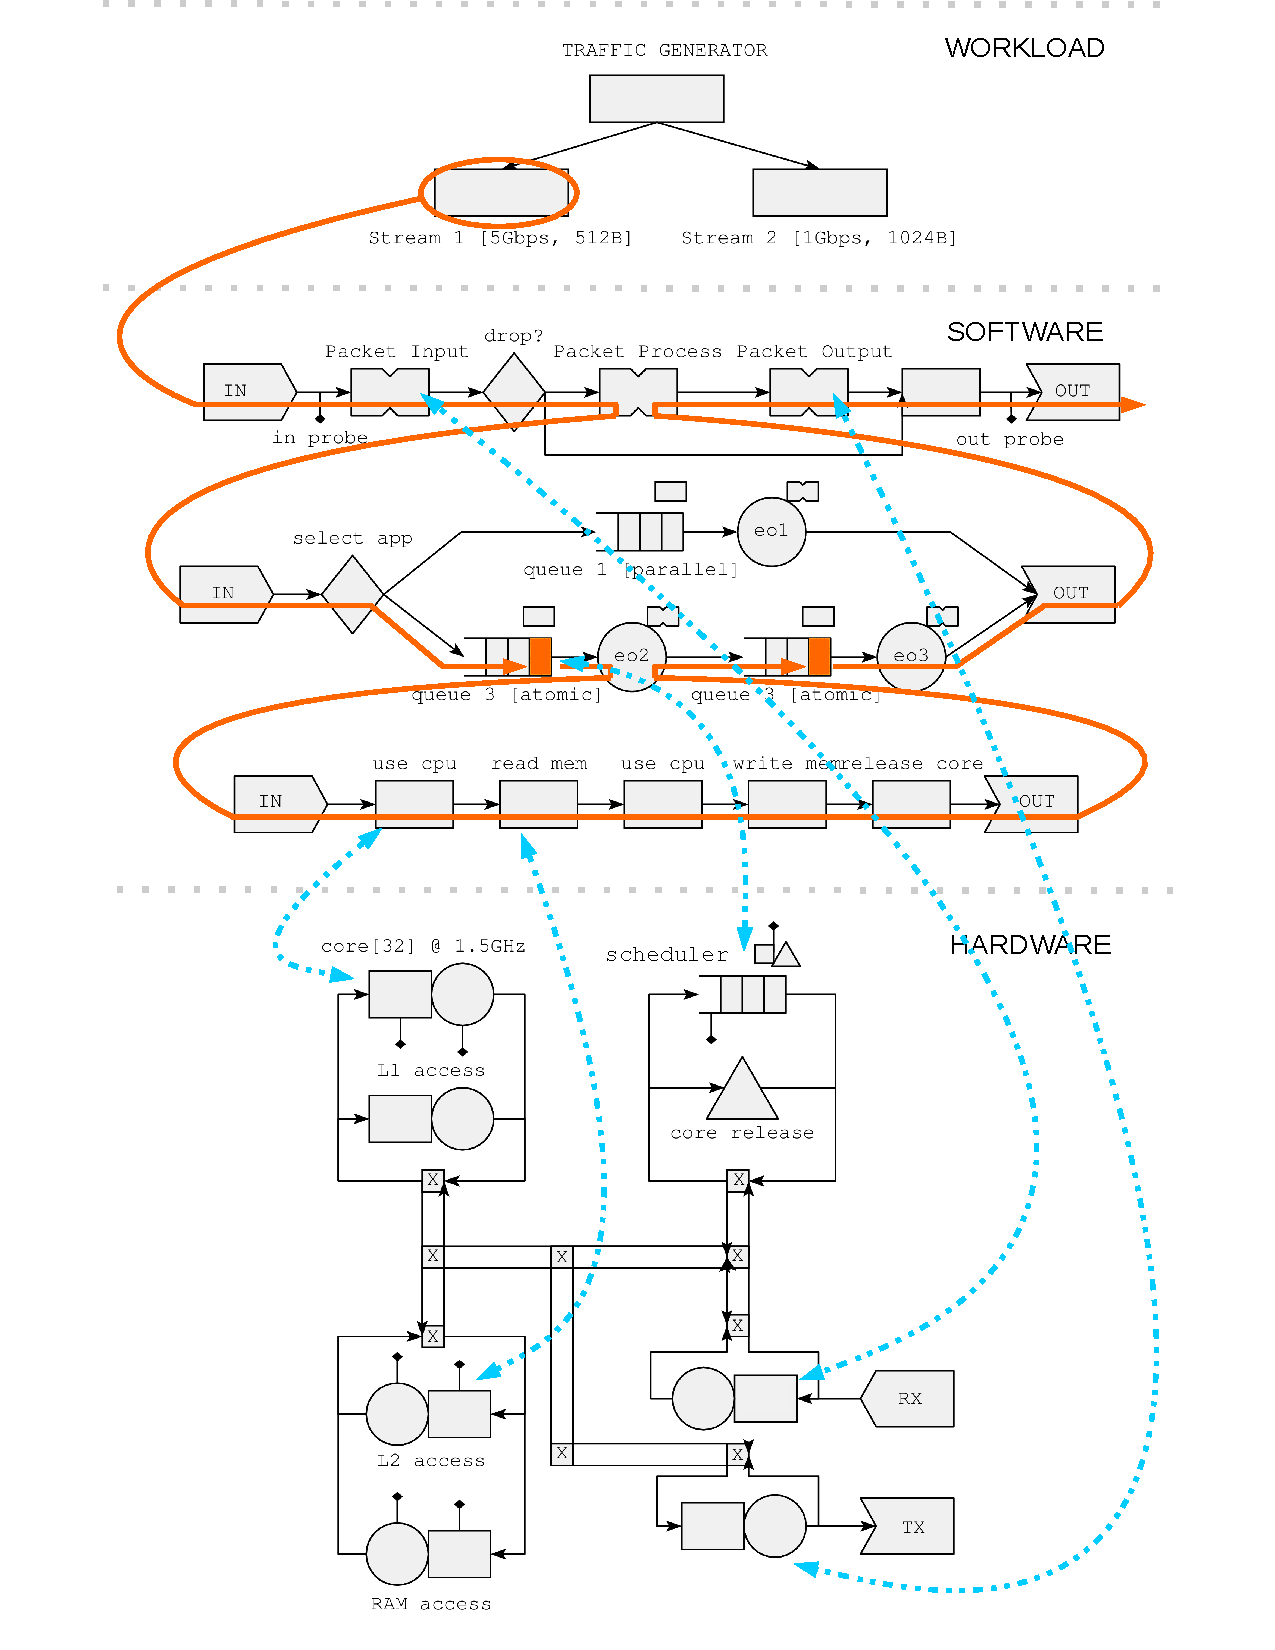
\includegraphics[width=\textwidth]{images/pse-models/fullmodel.pdf}
    \caption{Graphical presentation of the PSE model of a network processing system. The workload model (top) generates network packets, which then flow through the software model (middle), consuming the hardware resources (bottom). The orange arrows represent an example of a packet's path through the software model, and the blue arrows the resource usage at each software model node.}
    \label{fig:full-model}
  \end{center}
\end{figure}

The workload model, at the top of the picture, consists of two packet streams. The \emph{TRAFFIC GENERATOR} node activates the two stream nodes, which again generate packets that enter the software layer. The workload nodes contain parameters, such as the application id's, that are used to control the packet flows in the software model.

% has a lifetime of 0.5 seconds, and it triggers the streams with interval drawn from a uniform distribution with parameters 0.00005 and 0.00015. The streams have lifetime of 0.0004 seconds, and interval drawn from a lognormal distribution. The packet sizes of the streams are defined with the size attribute. Both of the streams also specify an appId attribute that is used to define the processing application in the software model. The packets from both streams enter the IN node of the top level software model.

The software model is divided into several submodels. The top software level model consists of packet input, packet processing and packet output submodels. The submodel view of the packet input and packet output are omitted from the picture for the sake of simplicity, as in both of these phases, the core and memory usage is linearly dependent on the packet size with additional Gaussian noise. In the input phase, the packet consumes specific amount of core cycles for the header processing, and copies the packet header and the packet data to the memory. Packet output node copies the packet from the memory, and consumes certain amount of clock cycles for the packet checksum calculations.

The packet processing submodel is presented in the middle software layer. The select app node forwards each of the packets to one of the two packet processing application, based on the application id attribute defined in the workload model. The queue nodes represent the core scheduling done by the scheduler hardware unit. The packets arriving in the upper application have priority of 1, and they can be processed in parallel. In the application below, there are 2 atomic queues with priority 3. When the packet receives the passive resource from scheduler, it can enter the actual processing application, called execution object (eo). The execution objects are submodels that consume core cycles and memory similarly to the packet input and packet output submodels presented above. The scheduler/core passive resource is released inside each execution object.

The hardware model is a simple one level model containing no submodels. In the bottom left hand corner, there are PKI and PKO devices providing processor cycles for the packet input and packet output phases. The only passive resource node, scheduler, provides core access resources, which can be released with the core release node. The application cores are shown in the top left corner of the hardware layer. There are 32 cores, and a specific L1 cache access for each of them. The L2 and RAM memory resources provide the delay for reading and writing to memory.

The probes, attached to the scheduler unit, the cores, and the memory nodes, are used to gather statistics from the execution. Each of the units has two probes, one to measure the resource usage, and the other to measures the queue for the corresponding resource. In this hardware model, the routing nodes (squares) and the edges connecting the resources do not have any functional meaning.

\section{Modeling the Task Scheduler}
\label{sec:modeling-task-scheduler}
The scheduler unit has an important effect on the tasks' throughput times, as it controls the order in which the tasks get service from the application cores. This section first describes the application nodes used to model the scheduler unit, and then the actual plug-in functions used to implement the scheduling functionality on the hardware model level.

When modeling the applications on PSE, it is helpful to consider the flow from the task's perspective. When a task has passed the input processing, it is put into the scheduler queue to wait to be scheduled on the application cores. Each time a core finishes its previous task, it requests for a new work from the scheduler-unit, which then schedules a task based on the flow quality of service priority and work group.

\subsection{Application Models}
\label{application-models}

Each packet processing application consists of two parts: the scheduler queue node, and the actual processing. The software layer in Figure~\ref{fig:full-model} presents an example of two main applications. The second application is divided into two sub-applications. The parameters for the first application's queue and execution object are shown in the Listings~\ref{lst:queue-attributes} and~\ref{lst:eo-attributes}, respectively.

\lstinputlisting[caption=The attributes of the scheduler queue.,
                 label=lst:queue-attributes]{listings/queue-attributes.txt}

The first line in Listing~\ref{lst:queue-attributes} specifies the display title for the node, as shown in the Figure~\ref{fig:full-model}. The \emph{name} and \emph{type} attributes specify that the resource usage is passive, and the required resource provision entity is $core\_require$, i.e. the scheduler. The parameters on lines 5-7 define the parameters that are used in the custom scheduling code on the hardware level. The \emph{$queue\_type$} value atomic specifies that two nodes entering the scheduler from the same resource usage node, cannot be processed simultaneously. The \emph{$queue\_id$} is used to keep track of the tasks being processed, and \emph{$queue\_priority$} is used to globally prioritize tasks between the queues.

\lstinputlisting[caption=The attributes of execution object.,
                 label=lst:eo-attributes]{listings/eo-attributes.txt}

The execution object node parameters are shown in the Listing~\ref{lst:eo-attributes}. It is a simple submodel node. It specifies the display title, and the name of the submodel to be used. The \emph{file} attribute specifies the file that defines the submodel. Note that, each execution object submodel needs to release the scheduler/core resource, as shown in the Figure~\ref{fig:full-model}.

\subsection{Global Hardware Scheduler}
\label{sec:scheduler-unit}
To model the processing cores' run-to-completion behavior, the scheduler unit is modeled as a passive resource. Each time a task is entering a processing application, it first acquires the passive scheduler resource. The amount of available passive scheduler resources is equal to the processing cores in the system, and a task cannot use processing core without holding the scheduler resource.

The scheduler unit model requires the use of custom scheduling functions. These are modeled using PSE's custom plug-in interface, presented in Chapter~\ref{chapter:mechanism-for-extended-queue-disciplines}. The functionality is implemented in two custom functions, written in C-code: the selection function, and the reserve function. The resource node parameters are changed to use these functions. The parameters of the scheduler node used in the example model are presented in the Listing~\ref{lst:RNS-attributes}.

\lstinputlisting[caption=The attributes of the scheduler node to determine the custom scheduler.,
                 label=lst:RNS-attributes]{listings/scheduler-attributes.txt}

The first three lines specify the node title, name, and capacity. The capacity is set to the amount of available processing cores, meaning that no more than 32 tasks can be processed simultaneously. The \emph{discipline} parameter \mbox{CUSTOM}, on line 5, specifies that a custom scheduler is used instead of the built-in scheduling functions. The \emph{file} parameter specifies the path of the C header file that declares the scheduling functions. The \emph{$select\_function$} and the \emph{$reserve\_function$} parameters specify the two functions that are required to implement the scheduling logic.

The reserve function is called each time a task enters a resource usage node in the resource usage model, and it determines whether the task can immediately be served, or if it has to wait for the service. If the task can be processed immediately, it is inserted to the processing queue of the resource, and to the waiting queue otherwise. If the task gets put to the waiting queue, the reserve function also needs to reorder the queue.

Listing~\ref{lst:CUSTOM_reserve} describes the reserve function used to model the scheduler. The function takes four input arguments: \emph{r} contains the data of the resource being reserved; \emph{queue} is a pointer whose value is assigned either to the processing queue or the waiting queue; \emph{position} is a pointer, whose value is assigned to the position in the queue; \emph{$new\_client$} holds the parameters, defined in the workload and resource usage models, of the new task.

\lstinputlisting[caption=The $CUSTOM\_reserve$ function for scheduler.,
                 label=lst:CUSTOM_reserve]{listings/CUSTOM_reserve.c}

On the lines 11-39, the reserve function attempts to place the task in the processing queue. The if-statement, on line 11, checks if the resource capacity is full. If there are available cores, then the processing conditions are checked, by going through all the cores, as shown in the for-loop on lines 21-32. If the new task's flow is marked atomic (in the reserve node in resource usage graph), and another task from the same flow is being processed on one of the cores (if-condition on lines 25-26), then the for-loop breaks, and the task gets set to the waiting queue. If a core is not processing, and the flow's coremask permits processing on the core (if-condition on line 31), we assign core's index to variable \emph{j}. Finally, if there is available core (\emph{j} is smaller or equal than the resource capacity) and none of the tasks from the same atomic flow are being processed, we set the queue to point to the resource's processing queue, and the position to the variable \emph{j}, and return.

If the processing conditions are not met, i.e. the execution goes past the if-block, then the task is set into the waiting queue. Line 43 assigns the \emph{queue} to point to the waiting queue of the resource. The for-loop on lines 46-48 finds the first task with larger priority, at index \emph{i}, and the for-loop on lines 51-53 moves all the higher priority tasks one step further on the queue. Finally the index \emph{i} is assigned to \emph{position}, and the function returns.

Each time a core ends a processing of a task, a new task is selected for the processing, using the custom select function. Listing~\ref{lst:CUSTOM_select} shows the code used for the select function to model the scheduler.

\lstinputlisting[caption=The $CUSTOM\_select$ function for scheduler.,
                 label=lst:CUSTOM_select]{listings/CUSTOM_select.c}

$CUSTOM\_select$ takes the resource \emph{r}, and the index of the released core \emph{$release\_index$} as an input. The outer for-loop, starting at line 7, goes through all the tasks in the waiting queue, and finds the first task that satisfies the processing constraints, similarly as the reserve function. Line 10 checks if the waiting task's coremask allows the task to be processed on the core. If the waiting task's flow is atomic (line 12), we need to go through all the processing cores to check that there is no task being processed from the same flow (lines 18-24). If the task was not atomic, or no tasks from the same flow were being processed, the function returns the index of the task in the waiting queue. Otherwise we move to the next waiting task and repeat. If no task from the waiting queue can be scheduled, the function returns $RNS\_LARGE$. The RNS automatically moves the clients when it removes the task from the waiting queue.

%%% Local Variables:
%%% mode: latex
%%% TeX-master: "thesis-hartikainen"
%%% End:
